In this chapter, we mainly reintroduce important concepts from \citep{mining,discovery,efficient} for handling and modeling uncertain event data.
In particular, we show how these concepts enable conducting the tasks of process discovery and conformance checking on event data containing explicit uncertainty.
To accomplish this, uncertainty is incorporated in graph-type models which are then fed to existing methods for process discovery and conformace checking.
Given the corresponding event set of an uncertain process instance, uncertainty in any of the three attributes activity, timestamp and event type leads to potentially more than one possible event trace and activity trace related to that process instance.
Particularly, a consequence of timestamp uncertainty is that events may not be totally ordered in time.
Instead, they are only partially ordered.
In the following, we define the ``happened before'' relation over event pairs, which describes a strict partial order \cite{conformance}. 
%Since the case IDs serve to uniquely identify the process instances, in the remainder we often use the terms "case" and "process instance" interchangeably.

\begin{definition}[Strict partial order over uncertain events \cite{conformance}] \label{spo}
Let $e, e' \in \mathcal{E}$ be two uncertain events.
$(\prec_{\mathcal{E}},\mathcal{E})$ is an order defined on the universe of uncertain events as:
\begin{align*}
e \prec_{\mathcal{E}} e' \Leftrightarrow t_{max}(e) < t_{min}(e').
\end{align*}
\end{definition}

It is easy to prove that this binary relation is indeed a strict partial order.
In Proposition 1 in \cite{conformance} is shown that the relation is irreflexive and transitive.
The pairs of events which do not appear in the relation are uncomparable.
Lemma 1 from \cite{conformance} shows that uncomparable events share possible timestamp values.
In the remainder of this work, we often refer to such events as events with overlapping timestamps or simply overlapping events.

\begin{definition}[Correct evaluation orders \cite{conformance}]
Given a set $E \subseteq \mathcal{E}$ of uncertain events, a sequence $s \in \mathcal{S}_E$ is a \emph{correct evaluation order} for $E$ over $\prec_{\mathcal{E}}$ if and only if for all $1 \leq i < j \leq |E|$ we have that $s_j \not \prec_{\mathcal{E}} s_i$. 
\end{definition}

Note that given an uncertain process instance with corresponding event set $E$, a permutation over the events in $E$ is a correct evaluation order if and only if events which certainly happened in a particular order do not appear in the reversed order in the sequence.
The correct evaluation orders over $(E,\prec_{\mathcal{E}})$ are exactly the possible event sequences for the corresponding process instance \cite{conformance}.

\begin{definition}[Realizations of event traces]\label{def: event trace realizations}
Let $L$ be an uncertain log and $E$ be the set of events belonging to some case $c \in \mathcal{U}_C^L$.
%Let $\sigma_e$ denote the event trace of case $c$.
We define the set of \emph{event trace realizations of case $c$} as: 
\begin{align*}
\mathcal{R}_e(E) := \{
s_e \in \mathcal{S}_E \mid
s_e \text{ is a correct evaluation order for } E ~ over 
\prec_{\mathcal{E}}
\}.
\end{align*}
\end{definition}

\begin{definition}[Realizations of activity traces]\label{def: activity trace realizations}
Let $L$ be an uncertain log and $E$ be the set of events belonging to some case $c \in \mathcal{U}_C^L$.
%Let $\sigma_e$ and $\sigma_a$ be the event trace and activity trace of case $c$ respectively.
Let $\mathcal{R}_e(E)$ be the set of event trace realizations of $c$.
We define the set of \emph{activity trace realizations $c$} as: 
\begin{align*}
\mathcal{R}_a(E) = \{
 s_a \in A(s_e) \mid
s_e \in \mathcal{R}_e(E) 
 \}.
\end{align*}
\end{definition}


Note that for a case with no uncertainty in activities, each event trace realization enables the execution of a unique sequence of activities.
Otherwise, the same event trace might enable many possible activity traces.
If there are indeterminate events, then the possible event traces might contain different sets of events, which again affects the corresponding activity traces and their lengths.
Uncertainty in timestamps is particularly critical.
As a consequence, the events may not be totally ordered into a unique sequence, leading to potentially more than one ordering according to which the uncertain events might have been executed.
While obtaining the possible activity sequences from a given event sequence simply requires obtaining the cartesian product over the sets of  possible activities for each event, computing the possible event traces in the first place is computationaly more challenging.
For a set of $n$ events, there are $n!$ permutations, and each of those permutations is a potential event trace realization.
%In Section \ref{sec:realizations} we introduce a method on how to obtain these sequences.

\begin{definition}[Follows Graph]\label{def: follows graph}
Let $E$ be the event set belonging to a process instance from some uncertain event log $L$.
We construct the \emph{follows graph} $\mathcal{F}(E)=(V_{\mathcal{F}},E_{\mathcal{F}})$ of the event set $E$, where 
$V_{\mathcal{F}} = E \text{ and }
E_{\mathcal{F}} = \{(u,v) \in V_{\mathcal{F}} \times V_{\mathcal{F}} \mid 
u \prec_{\mathcal{E}} v \}.$
\end{definition}

In the follows graph $\mathcal{F}(E)$, there is a vertex for every event and an arc going from one vertex to another if their corresponding events certainly happened in a particular order (their time intervals do not overlap).
Fig. \ref{fig: fg1} shows the follows graph of the event set from Table \ref{table: table1}.
An arc between two vertices indicates that the corresponding event pair may be in a predecessor-successor relationship w.r.t. the time of execution.

\begin{lemma}\label{lemma: edge path}
Let $E$ be the event set of some case $c \in \mathcal{U}_C$, and let $\mathcal{F}(E)=(V_{\mathcal{F}},E_{\mathcal{F}})$ be the follows graph of $E$.
For every pair $u,v \in V_{\mathcal{F}}$ it holds that $u \mapsto v$ if and only if $(u,v) \in E_{\mathcal{F}}$.
\end{lemma}

\begin{proof} 
\leavevmode \\ 
$(\Leftarrow)$ Trivial, since every arc connecting two vertices is also a path between them. \\ \\
$(\Rightarrow)$ Suppose there is a path $p \in p_{\mathcal{F}(E)}(u,v)$ between $u$ and $v$ and $(u,v) \not \in E_{\mathcal{F}}$.
Because $p$ is a path, it holds that 
$\forall ~ 1 \leq i < |p|: ~ (p[i],p[i+1]) \in E_{\mathcal{F}}$.
By definition of $E_{\mathcal{F}}$, it follows that 
$\forall ~ 1 \leq i < |p|: ~ p[i] \prec_{\mathcal{E}} p[i+1]$.
Since $\prec_{\mathcal{E}}$ is a strict partial order, from transitivity follows that $\forall ~ 1 \leq i < j \leq |p|: ~ p[i] \prec_{\mathcal{E}} p[j]$, and especially $p[1]=u \prec_{\mathcal{E}} v=p[|p|]$.
This contradicts the assumption that there is no arc between $u$ and $v$.
%$\lightning$
%\qed
\end{proof}
\pagebreak

\begin{theorem}\label{theorem: topological sortings}
Let $E$ be the event set of some uncertain process instance and let $\mathcal{F}(E)$ be its follows graph.
Then, $\mathcal{F}(E)$ is acyclic and the set of all topological sortings of the follows graph corresponds to the set of event trace realizations: $\mathcal{O}_{\mathcal{F}(E)} = \mathcal{R}_e(E)$.
\end{theorem}

\begin{proof}
Suppose there is a cycle $(v_1,v_2,...,v_n,v_1) \in P_{\mathcal{F}(E)}$.
By definition, $(u,v)\in E_{\mathcal{F}(E)}$ if and only if $u \prec_{\mathcal{E}} v$.
Thus: $v_1 \prec_{\mathcal{E}} v_2, v_2 \prec_{\mathcal{E}} v_3, ..., v_n \prec_{\mathcal{E}} v_1$.
Since $\prec_{\mathcal{E}}$ is a strict partial order, from transitivity it follows that $v_1 \prec_{\mathcal{E}} v_1$.
This contradicts the irreflexivity of $\prec_{\mathcal{E}}.$

Let $s = \langle e_1,...,e_{|E|} \rangle \in \mathcal{S}_E$ be a permutation over the set of events $E$.
It holds that 
\begin{align*}
s \in \mathcal{O}_{\mathcal{F}(E)} 
&\overset{\text{Def.} \ref{def: topological sorting}}{\Longleftrightarrow} 
\forall ~ 1 \leq i < j \leq m: ~ s[j] \not \mapsto s[i] \\ 
&\overset{\text{Lem.} \ref{lemma: edge path}}{\Longleftrightarrow} 
\forall ~ 1 \leq i < j \leq m: ~
(s[j],s[i]) \not \in E_{\mathcal{F}} \\
&\overset{\text{Def.} \ref{def: follows graph}}{\Longleftrightarrow} 
\forall ~ 1 \leq i < j \leq m: ~
s[j] \not \prec_{\mathcal{E}} s[i] \\
&\overset{\text{Def.} \ref{eval}}{\Longleftrightarrow} 
 s \text{ is a correct evaluation order for } E~ over \prec_{\mathcal{E}} \\
&\overset{\text{Def.} \ref{def: event trace realizations}}{\Longleftrightarrow} 
s \in \mathcal{R}_e(E).
\end{align*} 
%\qed
\end{proof}


\begin{algorithm}[h!]
	\caption{\textsc{FollowsGraph($E$)}}
	\label{alg:follows graph}
	\SetKwInOut{Input}{Input~}
	\SetKwInOut{Output}{Output~}
	\Input{~An event set $E$.}
	\Output{~Follows Graph $\mathcal{F}(E)$.}
	
	$\mathcal{L} \gets \langle ~ \rangle$ \tcp*{Support list}
	
	$Arcs \gets \{~\}$ \tcp*{Set of arcs}
	
	\For{$e \in E$}{ \label{1: 3}
		$\mathcal{L} \gets \mathcal{L} \oplus (t_{min}(e),e,\text{'MIN'})$
		
		$\mathcal{L} \gets \mathcal{L} \oplus (t_{max}(e),e,\text{'MAX'})$
	} \label{1: 5}
	
	\textsc{Sort}$(\mathcal{L})$ \tcp*{Sorts the list based on timestamp value} \label{1: 6}
	
	$finished \gets \{ ~ \}$ \tcp*{Set of finished events}
	
	$i \gets 1$
	
	\While{$i \leq |\mathcal{L}|$}{ \label{1: 9}
		$(t,e,type) \gets \mathcal{L}[i]$
		
		\If{$type = \text{'MAX'}$}{ \label{1: 11}
			$finished \gets finished \cup \{e\}$ \label{1: 12}
		}
		\ElseIf{$finished \neq \{ ~ \}$}{ \label{1: 13}
			\For{$e' \in finished$}{
				$Arcs \gets Arcs \cup \{(e',e)\}$ \label{1: 15}
			}
		}
		$i \gets i+1$
	}
	
	\Return $\mathcal{F}=(E,Arcs)$
\end{algorithm}
\pagebreak

Algorithm \ref{alg:follows graph} shows how the follows graph can be computed for some given event set $E$.
At first, each event is stored twice in a support list, accompanied by either its minimum or maximum timestamp, together with the indication regarding the timestamp type (lines \ref{1: 3}-\ref{1: 5}).
Then, the support list is sorted based on these timestamp values in line \ref{1: 6}.
The arcs are defined the following way:
We scan through all events in line \ref{1: 9} and whenever we encounter an event with its maximum timestamp, we store it in the $finished$ set (lines \ref{1: 11}-\ref{1: 12}).
This means it is certain that the event has been executed until that point.
When we encounter an event with a minimum timestamp, an arc is added from all finished events to the current event (lines \ref{1: 13}-\ref{1: 15}).
This way we ensure that $(e',e) \in Arcs$ if and only if $e' \prec_{\mathcal{E}} e \Leftrightarrow t_{max}(e') < t_{min}(e)$, in accordance with Definition \ref{def: follows graph} of the follows graph.
The follows graph is returned in the end, containing the event set as nodes together with the computed arcs.

%
%
%
%
%
%
\begin{figure}[h]
	\centering
	{
	\begin{tikzpicture}[->,>=stealth',shorten >=1pt,node 						distance=2.5cm,auto,main node/.style={circle,draw,align=center}]
	%\draw [help lines] (0,0) grid (7,4);
	\node[main node,label=above: \large $a$] (A) at (1,2) {$e_1$};
	\node[main node,label=above: \large ${\{b,c\}}$] (B) at (3,3) {$e_2$};
	\node[main node,dashed,label=above: \large $d$] (C) at (3,1) {$e_3$};
	\node[main node,label=above: \large ${\{c,e\}}$] (D) at (5,3) {$e_4$};
	\node[main node,label=above: \large $e$] (E) at (5,1) {$e_4$};
	
	\path
	(A) edge (B)
	(A) edge (C)
	(A) edge [bend left=40](D)
	(A) edge [bend right=50](E)
	(B) edge (D)
	(B) edge (E)
	(C) edge (D)
	(C) edge (E)
	

	;
	\end{tikzpicture}
	\subcaption{The follows graph of the event set from Table \ref{table: table1}. Event pairs connected by an arc are in a predecessor-successor relationship regarding the time of their execution.
	}
	\label{fig: fg1}
	}
%
%
%
%
%
%
%
%
	{
	\begin{tikzpicture}[->,>=stealth',shorten >=1pt,node 						distance=2.5cm,auto,main node/.style={circle,draw,align=center}]
	%\draw [help lines] (0,0) grid (7,4);
	\node[main node,label=above: \large $a$] (A) at (1,2) {$e_1$};
	\node[main node,label=above: \large ${\{b,c\}}$] (B) at (3,3) {$e_2$};
	\node[main node,dashed,label=above: \large $d$] (C) at (3,1) {$e_3$};
	\node[main node,label=above: \large ${\{c,e\}}$] (D) at (5,3) {$e_4$};
	\node[main node,label=above: \large $e$] (E) at (5,1) {$e_4$};
	
	\path
	(A) edge (B)
	(A) edge (C)
	%(A) edge [bend left=40](D)
	%(A) edge [bend right=50](E)
	(B) edge (D)
	(B) edge (E)
	(C) edge (D)
	(C) edge (E)
	

	;
	\end{tikzpicture}
	\subcaption{The behavior graph of the event set from Table \ref{table: table1}. It can be obtained through the transitive reduction of the follows graph in Fig. \ref{fig: fg1}.
	}
	\label{fig: bg1}
	}
	\label{fig: fg1 and bg1}
\end{figure}
%
%
%
%
%
\begin{definition}[Behavior graph \cite{mining}]
Let $E \subseteq \mathcal{E}$ be a set of uncertain events. 
A \emph{behavior graph} is a function $bg: \mathcal{P}(\mathcal{E}) \to \mathcal{G}$ with $\mathcal{G}$ denoting the universe of graphs, such that $bg(E)$ yields the transitive reduction of the follows graph $\mathcal{F}(E)$.
\end{definition}

Fig. \ref{fig: bg1} shows the behavior graph of the event set from Table \ref{table: table1}.

Every follows graph is acyclic, therefore every behavior graph is also acyclic, since it contains a subset of the arcs of the follows graph.
Similar to the follows graph, the topological sortings of the behavior graph of an uncertain process instance correspond to the correct evaluation orders for its event set over $\prec_{\mathcal{E}}$, as shown in Theorem 1 in \cite{conformance}.
While the methods we introduce in Chapter \ref{chap:realizations} to obtain the set of event trace realizations do not construct behavior graphs, we often use them throughout this work to visualize uncertain instances.
The topology of the behavior graph nicely incorporates the timestamp uncertainty in an intuitive manner.
Whenever there is a vertex with more than one outgoing (or ingoing) arc, the events represented by the target (or source) nodes have overlapping timestamps and no arcs between them.
In contrast to the follows graph, where arcs connect events whenever they are in a predecessor-successor relationship ($\prec_{\mathcal{E}}$), the behavior graph visualizes the ``directly-follows'' relationship instead.
%Whenever there is an arc between two vertices, the corresponding pair of events might have happened consecutively.
Computing the behavior graph through the transitive reduction runs in $\mathcal{O}(n^3)$ in the worst-case scenario \cite{transitive}.
However, a novel method that runs in $\mathcal{O}(n^2)$ in the worst-case scenario is introduced in \cite{efficient}.
It is worth noting that the structure of behavior graphs is only affected by timestamp uncertainty.
Moreover, the elapsed time between any two comparable events has no effect on the graph structure, only their order is important \cite{space}.

Whenever we visualize uncertain process instances through their behavior graphs, we indicate indeterminate events by drawing their corresponding vertices as dashed circles (see event $e_4$ in Fig. \ref{fig: bg1}).
Additionally, for each event, its possible activities are indicated above the corresponding vertex.

Behavior graphs are also used in \cite{discovery} to obtain UDFGs (\textit{Uncertain Directly-Follows Graphs}) in the context of process discovery.
Similar to DFGs, UDFGs are directed graphs constructed for a given log, where the vertices represent the activities and arcs connect activity pairs that might have happened consecutively in some process instance from the log.
In event data without uncertainty, there is always a fixed number of times for how often two activities happen consecutively in the log. 
In the uncertain scenario, where there might be different possible event orderings and indeterminate events, one can obtain a minimum and maximum estimate for this value \cite{discovery}.
Similarly, given some uncertain event $e \in \mathcal{E}$ and activity $a \in \pi_a^{set}(e)$, if event $e$ has many possible activities or is indeterminate, then activity $a$ might or might not have been executed.
Again, one can determine this way a minimum and maximum number of executions for each activity in the log.
For every activity and activity pair, in \cite{discovery} the authors formalize how the minimum and maximum frequencies can be obtained from the behavior graphs.
Similar to the certain scenario, where one can filter out activities and arcs from the DFG of a process instance based on frequency thresholds, in  the uncertain scenario, one can determine four thresholds, two for the minimum and maximum frequency of activities, and two for the minimum and maximum frequency of the directly-follows relationships between activities.
Applying these thresholds to the UDFG of an uncertain event log removes all activities and arcs whose possible frequencies do not lie between the corresponding minimum and maximum thresholds.
One can then feed the resulting graph to process discovery methods based on directly-follows relationships to obtain a process model \cite{discovery}.


In process mining without explicit uncertainty, conformance checking methods assume that each process instance has a unique trace.
Its conformance to a given process model is quantified by e.g. using \textit{alignments} \cite{alignment}.
The alignment technique yields a conformance score for any given trace and a process model by quantifying the distinction between that trace and a replayable trace from the model that is most similar to it.
Measuring the conformance of an uncertain process instance which may have many possible corresponding traces becomes more challenging.
Since each one of those traces has its own conformance score, it is unclear how to determine the conformance score for the trace set as a whole.
Naturally, the best and worst scores yield lower and upper bounds on the conformance score \cite{conformance}.
One could also compute the average score, or describe the process instance as \textit{conforming} whenever at least one of its possible traces is replayable by the model, and \textit{non-conforming} otherwise \cite{por}.
In Chapter \ref{chap:estimates}, we compute an \textit{expected conformance score} by weighing the conformance score of each possible trace by its probability.

%
%
%
%\newpage
\begin{figure}[h!]
	\centering
	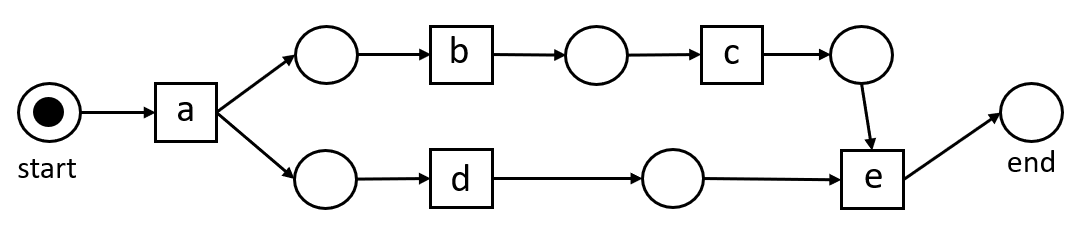
\includegraphics[width=0.8 \columnwidth]{figures/model1.png}
	\caption{A model of the process to which the case from Table \ref{table: table1} belongs. }
	\label{fig: model1}
	%width=1\columnwidth
\end{figure}
%
%
%
%
\begin{definition}[Petri Net]
A Petri Net is a tuple $N=(P,T,F)$ where $P$ is the set of places, $T$ the set of transitions, $P \cap T = \emptyset$ and $F \subseteq (P \times T) \cup (T \cup P)$.
A marking $M \in \mathcal{B}(P)$ is a multiset of places.
A Petri net $N=(P,T,F)$ defines a directed bipartite graph where $P \cup T$ is the set of vertices and $F$ is the set of arcs.
\end{definition}

A \textit{marking} describes the state of the Petri net and it indicates how many \textit{tokens} are contained in each place.
For any place or transition $x \in P \cup T$, $\bullet x=\{x' \mid (x',x) \in F\}$ denotes the set of its input nodes, whereas $\bullet x=\{x' \mid (x,x') \in F\}$ denotes the set of its output nodes.
Note that the input and output nodes of places can only be transitions and vice-versa.
A transition is \textit{enabled} if there is at least one token in each of its input places.
An enabled transition can \textit{fire}, an action which removes one token from each input place and adds one token to each output place.
Given two markings $M$ and $M'$, we say that marking $M'$ is \textit{reachable} from $M$ if there exist transitions $\ t_1,...,t_n $ and markings $M_0,...,M_n$ such that $M_0=M$, $M_n=M'$, and for all $1 \leq i \leq n $: transition $t_i$ is enabled in $M_{i-1}$ and firing $t_i$ results in marking $M_i$.
In this case, we also say that $M'$ is reachable from $M$ through the firing sequence $\langle t_1,...,t_n \rangle$.

\begin{definition}[Labeled Petri Net]
A labeled Petri Net $N=(P,T,F,\ell)$ is a Petri Net $(P,T,F)$ with a labeling function $\ell: ~ T \not \to \mathcal{U}_A$ which maps transitions to activity labels.
Given two markings $M$ and $M'$, we say $M'$ is reachable from $M$ through some activity sequence $\sigma_A$ if and only if there is a firing sequence $\sigma_T$ such that $M'$ is reachable from $M$ through $\sigma_T$ and $\ell(\sigma_T)=\sigma_A$.
\end{definition}
Note that the labeling function is a partial function.
The transitions which are not assigned a label from $\mathcal{U}_A$ are called \textit{silent transitions} and we use the symbol $\tau$ to identify them.

\begin{definition}[System Net]
A System Net is a triplet $SN=(N,M_{init},M_{final})$ where $N=(P,T,F,\ell)$ is a labeled Petri net, $M_{init} \in \mathcal{B}(P)$ is the initial marking, and $M_{final} \in \mathcal{B}(P)$ is the final marking.
Set $\phi(SN)$ contains all activity sequences through which $M_{final}$  is reachable from $M_{init}$.
\end{definition}

In process mining, we usually refer to any system net $(N,M_{init},M_{final})$ as a Petri net with initial marking $M_{init}$ and final marking $M_{final}$.
We also call $\phi(SN)$ the set of \textit{replayable traces}.
Many process discovery algorithms applied on event data yield models in the form of Petri nets.
The quality of those models depends on their simplicity, the degree in which the replayable traces replicate exactly the traces from the log (\textit{fitness} and \textit{precision}), and so on.
\pagebreak

\begin{definition}[Behavior Net \cite{conformance}] \label{def: bn}
Let $E \subseteq \mathcal{E}$ be the event set corresponding to some uncertain process instance, and let $bg(E)=(V,Arcs)$ be its behavior graph.
A behavior net $bn: \mathcal{P}(\mathcal{E}) \to \mathcal{U}_{SN}$, where $\mathcal{U}_{SN}$ denotes the universe of system nets is a system net $bn(E)=(P,T,F,\ell,M_{init},M_{final})$ such that:\\
-$P= Arcs \cup  \\
\{(\textsc{start,v}) \mid \nexists_{v'\in V} s.t. (v',v) \in Arcs\} \cup  \\
\{(\textsc{v,\textsc{end}}) \mid \nexists_{v'\in V} s.t. (v,v') \in Arcs\}$\\
-$T=\{(v,a) \mid v \in V \wedge a \in \pi_a^{set}(v)\} \cup \\
\{(v,\tau) \mid v \in V \wedge (\pi_o(v) = ? \vee \pi_o(v)=f_O \wedge f_O(?)>0 \}$ \\
-$F= \{((\textsc{start},v_1),(v_2,a)) \in Arcs \times T \mid v_1 = v_2\} \cup \\
\{((v_1,a),(v_2,w)) \in T \times Arcs \mid v_1=v_2\} \cup \\
\{((w,v_1),(v_2,a)) \in Arcs \times T \mid v_1=v_2\} \cup \\
\{((v_1,a),(v_2,\textsc{end})) \in T \times Arcs \mid v_1 = v_2\} $\\
-$\ell=\{((v,a),a) \mid (v,a) \in T \wedge a \neq \tau\}$ \\
-$M_{init} = [(\textsc{start},v) \mid v \in V]$ \\
-$M_{final} = [(v,\textsc{end}) \mid v \in V]$.
\end{definition}


Similar to the behavior graph, the behavior net is a model that incorporates the uncertaity of a process instance.
According to the definition of the behavior net, given an event set $E$, there is a transition $(e,a)$ for every $e \in E$ and $a \in \pi_a^{set}(e)$.
If $e$ is an indeterminate event, then there is an additional silent transition $(e,\tau)$ in the behavior net.
All transitions related to the same event $e \in E$ appear in an XOR construct, signaling an explicit choice.
For every arc $(e,e')$ in the behavior graph of event set $E$, there is a place connecting all transition pairs related to event $e$ and $e'$.
Since events with overlapping timestamps share a common predecessor in the behavior graph, their corresponding transitions appear in an AND construct in the behavior net.
It is shown in \cite{conformance} that the behavior net of an uncertain event set $E$ can replay all and only the activity trace realizations of $E$, that is: $\phi(bn(E)) = \mathcal{R}_a(E)$. 

The concept akin to the behavior net for certain process instances is the so-called \textit{event net}, which for a certain trace $\sigma$ of length $n$ contains $n$ visible transitions and $n+1$ places connected in a sequence.
The event net can only replay trace $\sigma$.
Note that the behavior graph of a certain trace is always a path of length $n-1$, containing $n$ vertices (one for each event) and $n-1$ arcs.

Next, we introduce the concept of \textit{alignment} \cite{alignment}, which we later use to determine a conformance score between a trace and a given model.
\begin{definition}[Alignment]
Let $SN=(N,M_{init},M_{final})$ be a system net with $N=(P,T,F.\ell)$ 
and let $\sigma_L \in \mathcal{U}_A^*$ be some arbitrary trace.
An alignment between trace $\sigma_L$ and system net $SN$ is a pair $(\sigma_L^{\gg},\gamma_M^{\gg})$ with $\sigma_L^{\gg} \in (\mathcal{U}_A \cup \{\gg\})^*$ and $\gamma_M^{\gg} \in (T \cup \{\gg\})^*$, such that the following hold:
\begin{align*}
&-\sigma_L^{\gg} \downharpoonright_{\mathcal{U}_A} = \sigma_L,\\
&-\gamma_M^{\gg} \downharpoonright_T = \gamma_M \text{ such that }M_{final} \text{ is reachable from } M_{init} \text{ through firing sequence } \gamma_M,\\
&-|\sigma_L^{\gg}| = |\gamma_M^{\gg}| = n \text{ and for } 1 \leq i \leq n \text{ one of the following holds: }
\sigma_L^{\gg}[i] = \ell(\gamma_M^{\gg}[i]), \\
&\gamma_M^{\gg}[i] = \gg \text{ or }   \sigma_L^{\gg}[i] = \gg.
\end{align*}
\end{definition}
%
%
%
%
%\newpage
\begin{figure}[h!]
	\centering
	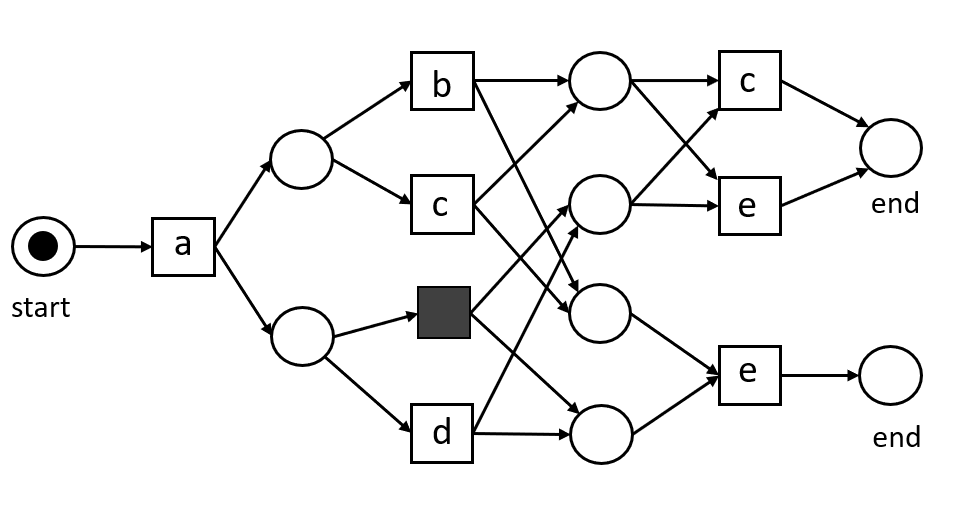
\includegraphics[width=0.8 \columnwidth]{figures/bn1.png}
	\caption{The behavior net corresponding to the event set from Table \ref{table: table1}. It can be constructed from the behavior graph shown in Fig. \ref{fig: bg1}.}
	\label{fig: bn1}
	%width=1\columnwidth
\end{figure}
%
%
%
%
%
\pagebreak
Alignments are used in conformance checking, and describe a correspondence between a trace $\sigma_L$ from some log $L$ and a process model $M$, where each position in the alignment indicates a \textit{move}.
All the matching positions between the two sequences $\sigma_L^{\gg}$ and $\sigma_L^{\gg}$ as defined above indicate the similarities between trace $\sigma_L$ from the log and trace $\ell(\gamma_M)$ which is replayable in the model.
These moves are called the \textit{synchronous} moves.
If in a particular position, sequence $\sigma_L^{\gg}$ contains symbol $\gg$, whereas $\gamma_M^{\gg}$ does not, this indicates a \textit{move only in the model}, implying that a particular behavior in the model is not replicated in the trace.
Similarly, if in a particular position, sequence $\gamma_M^{\gg}$ contains symbol $\gg$, whereas $\sigma_L^{\gg}$ does not, this indicates a \textit{move only in the log}, implying that a particular behavior in the trace is not replicated in the model.
The \textit{cost} of an alignment depends on the number non-synchronous moves.
Usually, we assign cost 1 to \textit{only log moves} and \textit{only model moves}, and cost 0 otherwise.
While there might be more than one alignment between a trace and a model, the conformance score is determined by the cost of the optimal alignment between them, that is, the alignment with minimal cost.
Such alignment describes how well the trace can be fitted in the model.
An alignment of cost 0 indicates that the trace is conforming to the model.
Not only do alignments provide a value quantifying conformance, but they also provide diagnostics by explicitly showing where a trace and a model deviate.
%
%
\begin{figure}[t]
  \centering
 {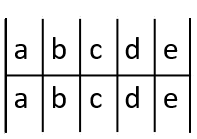
\includegraphics[width=30mm]{figures/align1.png}\label{align1}
	\subcaption{Optimal alignment between trace $\langle a,b,c,d,e \rangle$ and model from Fig. \ref{fig: model1} with cost 0.}
 	}
  %\hspace{2cm}
  {\label{align2}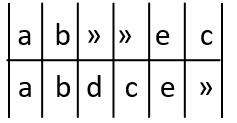
\includegraphics[width=36mm]{figures/align2.png}
	\subcaption{Optimal alignment between trace $\langle a,b,e,c \rangle$ and model from Fig. \ref{fig: model1} with cost 3.}
	}
	\label{fig: two alignments}
	\caption{Optimal alignments for two trace realizations of process instance from Table \ref{table: table1}.
	The projections of the first rows onto activity labels yield the two possible trace realizations, whereas the projections of the second rows onto activities yield the corresponding most similar traces replayable from the model shown in Fig. \ref{fig: model1}.}
\end{figure}
%

In this work, we also use the cost of optimal alignments as a measure for the conformance scores of possible trace realizations of uncertain process instances.
%
%
%
%
%
%
%